
\chapter{Wellenausbreitung}
Elektromagnetische Wellen breiten sich nicht überall gleich gut und auf die selbe Art und Weise aus. Die Frequenzwahl ist daher entscheidend für erfolgreiche Verbindungen.

Mit hohen Frequenzen kommt man grundsätzlich weiter als mit tiefen Frequenzen. Bei Nacht ist die \link{MUF}, bedingt durch die dünnere $\mathrm F_2$-Schicht, geringer.

\section{Die Ionosphäre}
Die Ionosphäre ist für HF-Funk von grosser Bedeutung. An ihr werden elektromagnetische Wellen reflektiert und gedämpft, und weltweiter Empfang wird erst möglich. Sie verändert sich mit der Sonneneinstrahlung und dem elfjährigen Sonnenfleckenzyklus.

\begin{figure}[h!]
 \centering
 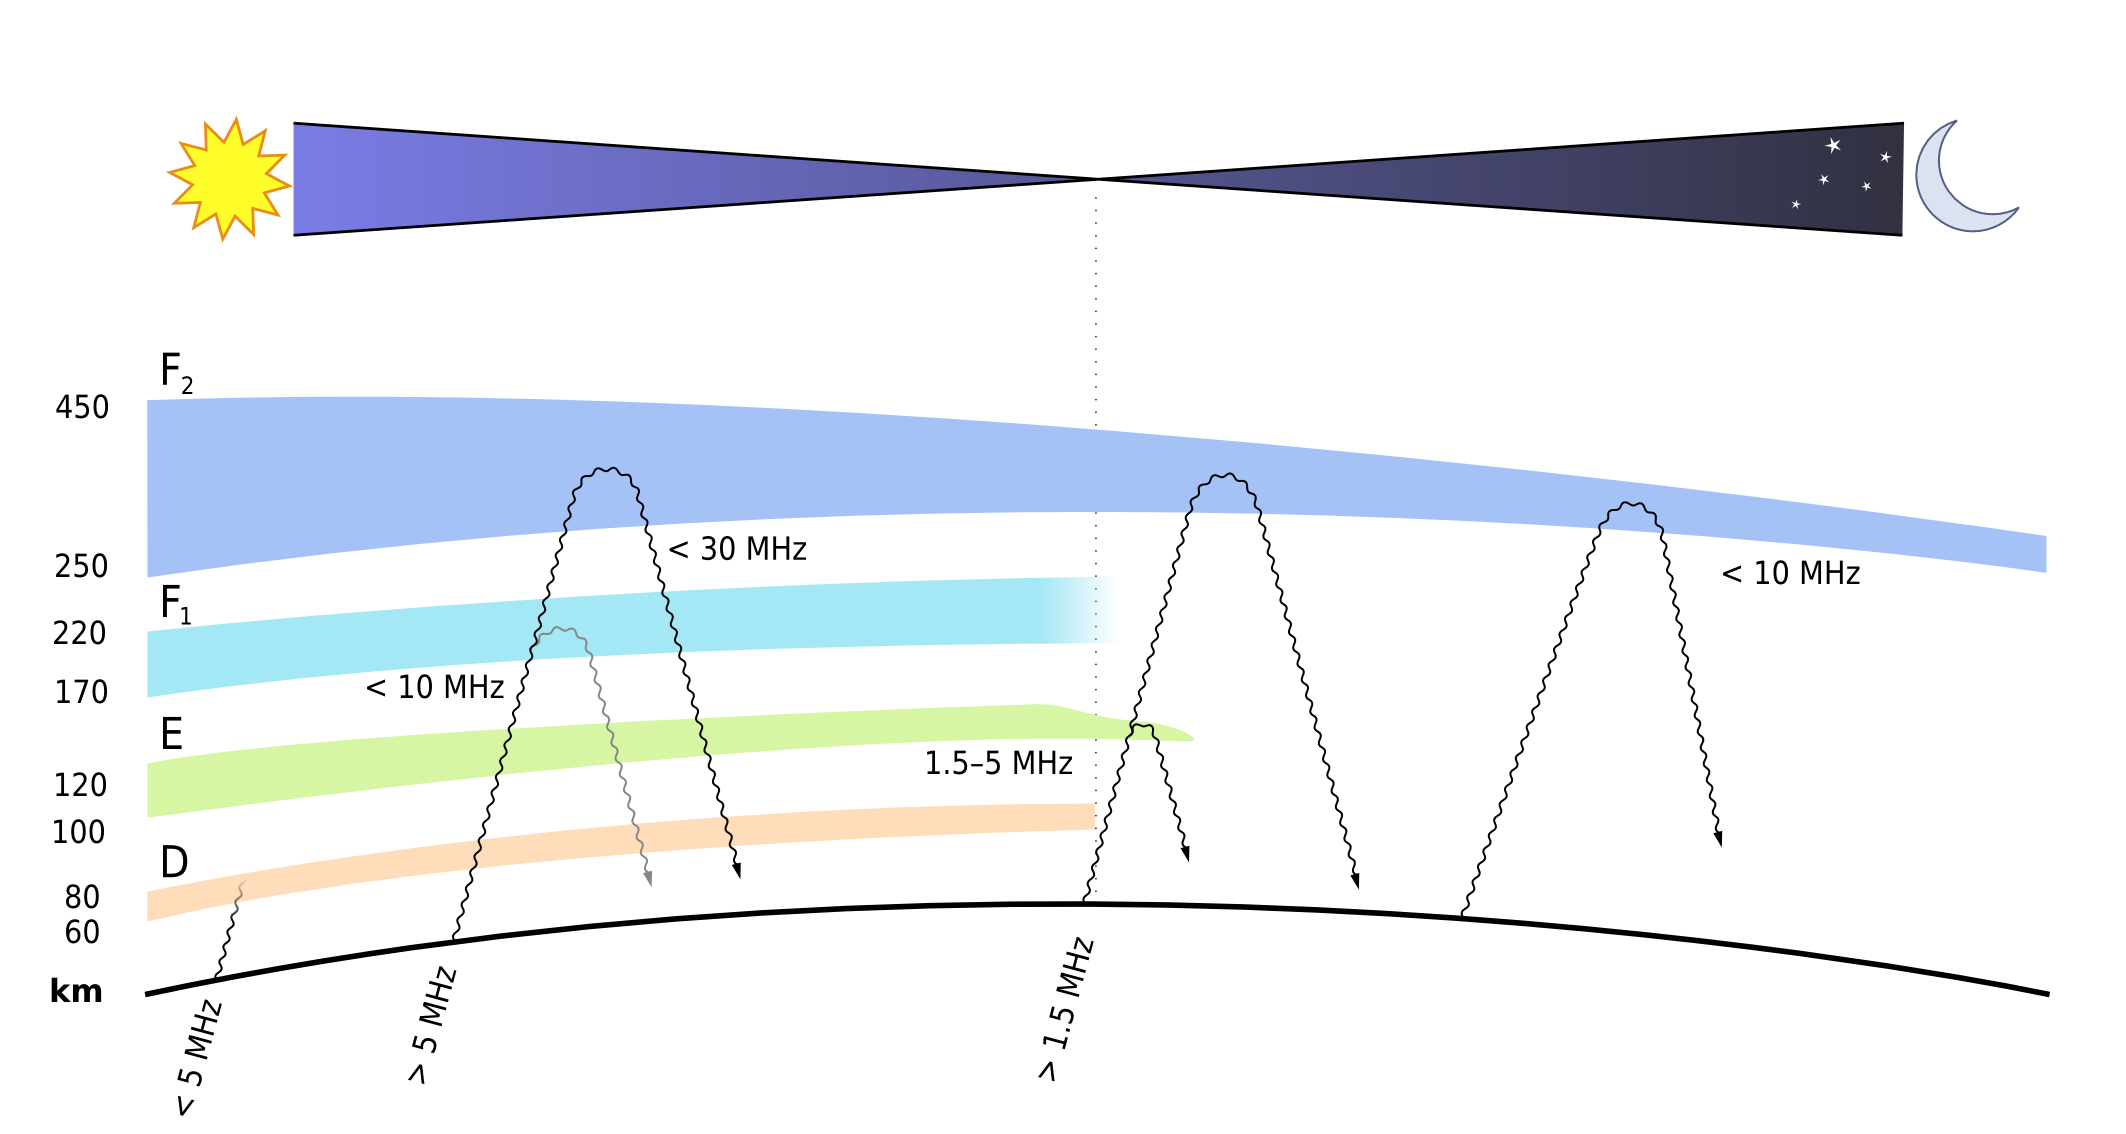
\includegraphics[width=11cm]{./png/Amfu-Ionosphere.png}
 \caption{Aufbau der Ionosphäre und reflektierende Eigenschaften der Schichten}
 \label{fig:ionosphere}
\end{figure}


Insgesamt besteht die Ionosphäre aus drei Schichten, die D-, E- und F-Schichten genannt werden. Die D-Schicht dämpft, die E-Schicht reflektiert tiefere Frequenzen und die F-Schicht höhere. Bei Sonneneinstrahlung (d. h. am Tag) werden Moleküle in der Ionosphäre durch Röntgen- und EUV\footnote{EUV: Extreme ultraviolette Strahlung mit Wellenlängen von 14 bis 80 nm}-Strahlung ionisiert. Eine weitere Rolle spielt die Sonnenfleckenzahl, die sich 2007 in einem Minimum befand und alle 11 Jahre ein Maximum erreicht. Je mehr Sonnenflecken vorhanden sind, desto stärker wird die Ionosphäre bei Sonneneinstrahlung ionisiert. Der Einfluss der Sonnenflecken ist nicht zu vernachlässigen; so sind HF-Frequenzen ab etwa 20 MHz während eines Minimums nicht verwendbar, in einem Maximum jedoch können weltweite Verbindungen beinahe den ganzen Tag entstehen.

\subsection{D-Schicht}
Die unterste der ionisierten Schichten existiert nur am Tag und reflektiert keine Signale. Tiefe Frequenzen unter 5 MHz werden so stark gedämpft, dass das 80-m- und das 160-m-Band nicht mehr benutzbar ist, auf höhere Frequenzen hat es keine grossen Auswirkungen.

Nach Sonnenuntergang verschwindet die D-Schicht sehr schnell, da die Ionen aufgrund der hohen Konzentration schnell wieder rekombinieren.

Bei sehr starker Sonnenaktivität kann der sogenannte \textit{Mögel-Dellinger-Effekt} auftreten. Dann ist die D-Schicht so stark ionisiert, dass das gesamte HF-Band für einige Minuten bis Stunden mehr oder weniger tot ist.

\subsection{E-Schicht}
Tagsüber dämpft die E-Schicht Frequenzen über 5 MHz, da die Ionenkonzentration für eine Reflexion zu gering ist. Tiefere Frequenzen werden reflektiert, müssen aber zuerst die D-Schicht passieren. Die Ionisierung befindet sich um die Mittagszeit in einem Maximum und verringert sich danach wieder langsam.

Nach Sonnenuntergang rekombiniert die E-Schicht innerhalb ungefähr einer Stunde nahezu vollständig. Innerhalb dieser Stunde kann sie für kurze Verbindungen über 500 km genutzt werden, da das 80-m- und 160-m-Band dann nicht mehr durch die D-Schicht gesperrt ist.

Im Sommer tritt manchmal manchmal die \textit{Sporadische E-Schicht} ($\textrm E_S$) auf. Es ist nicht klar, wie sie entsteht. An ihr wird sogar VHF reflektiert, was Überreichweiten und hohe Signalstärken ermöglicht. HF wird an einer tieferen Schicht als sonst reflektiert und erlaubt so Verbindungen über kürzere Distanzen von unter 500 km \textit{(Short Skip)}.

\subsection{F-Schicht}
Die F-Schicht ist die wichtigste für HF. Sie besteht am Tag aus zwei verschiedenen Schichten: Der $\mathrm F_1$- und der $\mathrm F_2$-Schicht. In der $\mathrm F_1$-Schicht werden neue Ionen gebildet, die stärkste Ionenkonzentration befindet sich in der $\mathrm F_2$-Schicht. 

Da sich in der Region der $\mathrm F_2$-Schicht nur noch wenige Gasmoleküle befinden, benötigen die Ionen sehr lange zur Rekombination. Sie besteht darum auch während der Nacht, die Stärke nimmt aber ab und somit auch die \link{MUF}.

\section{Arten der Wellenausbreitung}
\subsection{Bodenwelle} \label{sec:bodenwelle}
Die Bodenwelle \textit{(Ground Wave)} hat bei LF eine Reichweite von über 400 km\footnote{Bei gebirgigem Gelände etwa die Hälfte, bei Ozeanen u. ä. mehr als das Zweifache.}, bei HF reicht sie jedoch auf 80 m knapp 150, auf 10 m nur noch um die 30 Kilometer weit. Sie bewegt sich in der Troposphäre über dem Boden und wird hauptsächlich vom Boden gedämpft. Dabei wirken sich zum Beispiel dichte Vegetation (Wald), trockener Boden und stark bebaute Gebiete negativ auf die Reichweite aus, was aber zum Beispiel bei militärischen Einsätzen gewünscht sein kann. Gut leitende Untergrunde wie Wasser führen zu grösseren Reichweiten.

\subsection{Raumwelle}
Mit der Raumwelle \textit{(Sky Wave)}, die wie die Bodenwelle von jeder HF-Antenne erzeugt wird, ist es möglich, durch (Mehrfach-)Reflexionen an der Ionosphäre grössere Distanzen zu überbrücken. Pro Hop (Reflexion auf der Erde) können mehrere hundert Kilometer zurückgelegt werden, sogar bei Nacht noch über 500. Bei jeder Reflexion wird das Signal gedämpft.

Je flacher der Abstrahlwinkel der Antenne ist, desto höhere Frequenzen kann man verwenden und desto weiter kommt man mit einem Hop. Umgekehrt sollte für eine Nahverbindung eine tiefe Frequenz und ein steiler Abstrahlwinkel über 30° gewählt werden.

Für Verbindungen über weite Entfernungen eignen sich die Stunden um Sonnenauf- und -untergang am besten, da zu dieser Zeit die F-Schicht zwischen den Stationen gut aufgebaut ist. Beispiel: Bei Verbindungen in die USA gegen den Mittag wäre dort Nacht und die F-Schicht sehr dünn, so dass diese Frequenzen nicht reflektiert würden. Um Sonnenuntergang wird die F-Schicht hier langsam abgebaut, über dem Atlantik ist sie am stärksten, und in den USA wird sie gerade aufgebaut.

Die Raumwelle wird ab VHF zur Space Wave.

\subsection{Space Wave}
Die \textit{Space Wave} tritt ab VHF aufwärts auf. Sie bewegt sich quasi-optisch, also ungefähr bis zum Horizont, da sie kaum gebeugt wird und dann im All verloren geht. Allerdings wird sie zum Beispiel an Bergen reflektiert und von Wäldern und Häusern gedämpft, wodurch ihre Reichweite um einiges eingeschränkt wird. 

\section{QRN – Störungen in der Atmosphäre}
Vor allem unterhalb des 20-m-Bandes können atmosphärische Störungen eine solche Stärke erreichen, dass Gegenstationen trotz hoher Signalstärke nur noch schlecht hörbar sind. Im Sommer nimmt das QRN aufgrund häufigerer Blitzentladungen zu.

\subsection{Blitze}
Während der Entladung eines Blitzes entsteht ein elektromagnetischer Puls, da sich während einer kurzen Zeit extreme Spannungsänderungen vollziehen und gewaltige Ströme fliessen. Solche Störungen lassen sich in sehr weiter Distanz noch messen. Mit speziellen Systemen ist es sogar möglich, die Blitze zu orten. So können ungefähr 95\,\% der Blitze festgehalten werden.

Die von Blitzen erzeugten Signale werden \textit{Spherics}, \textit{Tweeks} oder \textit{Whistler} genannt, je nachdem, wie weit sie «gereist» sind. Spherics erzeugen im Wasserfalldiagramm nur Striche, Tweeks leicht gebogene Striche und Whistler hinterlassen Kurven, da Frequenzen höherer Wellenlänge schneller sind und so früher ankommen. Tweeks und Whistler sind als Pfeifton hörbar, dessen Frequenz sich ändert. Bei Tweeks dauert dies ein paar Hundertstelssekunden, Whistler wandern entlang des Erdmagnetfeldes und sind aufgrund der noch grösseren zurückgelegten Distanz länger hörbar – bis mehrere Sekunden lang. Sferics sind als kurzes Knacken hörbar.

\begin{figure}[h!]
 \centering
 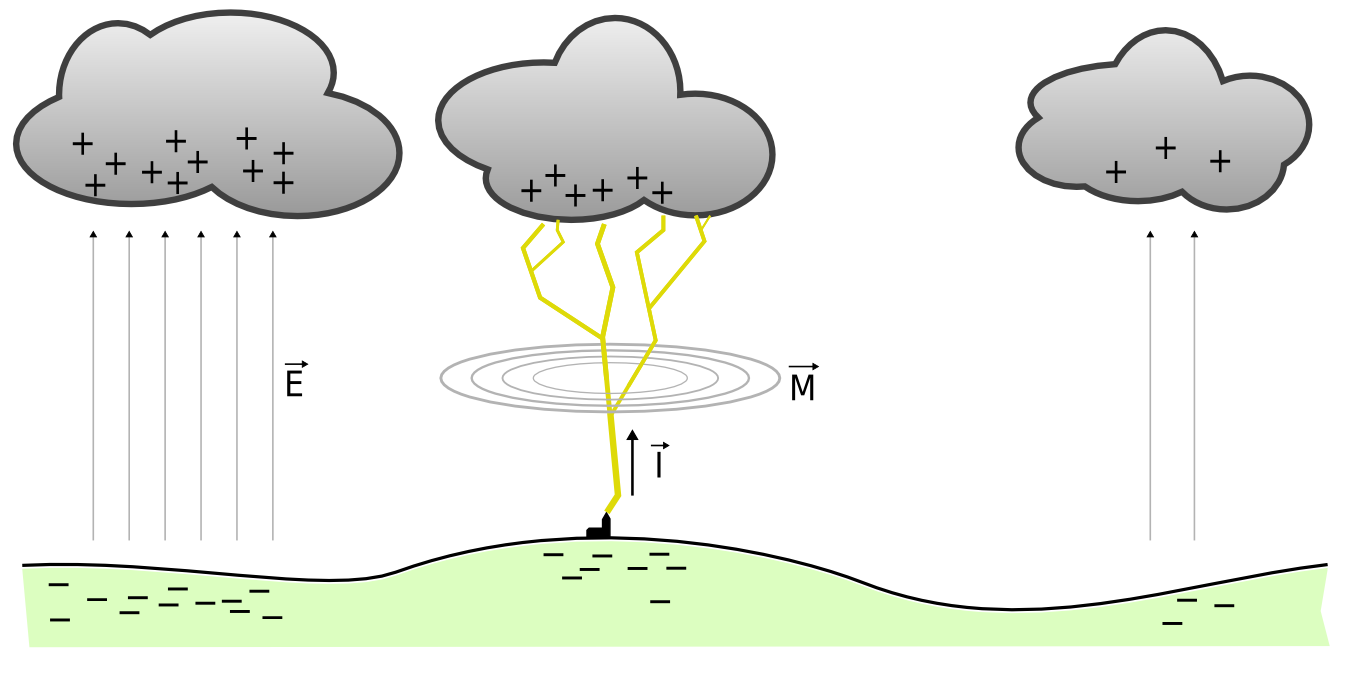
\includegraphics[width=11cm]{./png/Amfu-Blitz.png}
 \caption{Entladung eines Blitzes: Bei einem Gewitter besteht durch den Ladungsunterschied zwischen Wolke und Erde ein elektrisches Feld. Bei einem Blitz fliessen Elektronen (d. h. ein starker Strom) zur hier positiv geladenen Wolke, dadurch entsteht kurzfristig ein starkes magnetisches Feld.}
 \label{fig:blitz}
\end{figure}


Entladungen, die sich in der Nähe ereignen, erzeugen Störungen über das ganze Spektrum, hörbar in den unteren Bändern als starkes Knacken, in den oberen als kurz stark erhöhtes Rauschen.

\begin{figure}[h!]
 \centering
 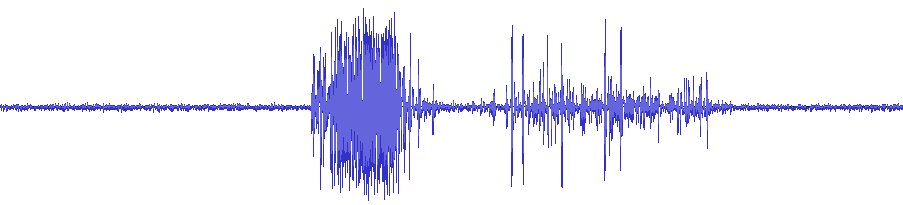
\includegraphics[width=5cm]{./png/Blitz-20M.png}
 \caption{Störung durch einen Blitz auf 21 MHz (Dauer des Ausschnittes: 2 Sekunden)}
 \label{fig:flash20}
\end{figure}


\section{QRM – Von Menschen verursachte Störungen}
QRM kann viele Ursachen haben. Auf Bändern mit hohem Funkverkehr können es ganz einfach andere Stationen sein, die so weit entfernt sind, dass sie nicht mehr verstanden, aber dennoch empfangen werden können und so den eigenen Funkverkehr stören. 

Eine andere häufige Störungsursache sind elektrische Geräte wie Computer, die in der Nähe laufen.



